% This is a sample LaTeX input file.  (Version of 11 April 1994.)
%
% A '%' character causes TeX to ignore all remaining text on the line,
% and is used for comments like this one.

\documentclass[11pt]{article}      % Specifies the document class
\usepackage{amsfonts,amssymb,amsmath}
\topmargin-0.2in
\textheight9.0in
\oddsidemargin-0.2in
\evensidemargin-0.2in
\textwidth6.5in

\usepackage{graphicx} % Required for inserting images
\usepackage{booktabs}
\usepackage{subcaption}
\usepackage{xcolor}  

\usepackage{listings}
\lstset{
	basicstyle=\footnotesize\ttfamily,
	columns=flexible,
	breaklines=true,
	commentstyle=\color{red},
	keywordstyle=\color{black}\bfseries}

\newcommand{\mZ}{\mathbb Z}
\newcommand{\mR}{\mathbb R}
\newcommand{\mC}{\mathbb C}
\newcommand{\mQ}{\mathbb Q}
\newcommand{\ep}{\epsilon}
\begin{document}             % End of preamble and beginning of text.

%\thispagestyle{empty}
\begin{center}
{\bf\large HW3(FEA): Appiah Francis}\\
\vspace{0.05in}
\end{center}
%--- coding
\begin{enumerate}
\item[I(iii)] This is the numerical results for (i), where $x_k=0.5$ is a node.
\begin{table}[!h]
	\caption{Errors and convergence orders for $k_1=1$, $k_2=5$}
	\vspace{0.1in}
	\centering
	\begin{tabular}{|c|c|c|c|c|}
		\hline
		$N+1$ & $||e_h||_{L^2}$ & Order & $||e_h||_{L^\infty}$ & Order \\
		\hline
		10  & 6.5420E-04 & --   & 1.1111E-03 & --   \\
		20  & 1.6355E-04 & 2.00 & 2.7778E-04 & 2.00 \\
		40  & 4.0888E-05 & 2.00 & 6.9444E-05 & 2.00 \\
		80  & 1.0222E-05 & 2.00 & 1.7361E-05 & 2.00 \\
		160 & 2.5555E-06 & 2.00 & 4.3403E-06 & 2.00 \\
		\hline
	\end{tabular}
	\label{tab:k1_1_k2_5}
\end{table}
\begin{table}[!h]
	\caption{Errors and convergence orders for $k_1=3$, $k_2=10$}
	\vspace{0.1in}
	\centering
	\begin{tabular}{|c|c|c|c|c|}
		\hline
		$N+1$ & $||e_h||_{L^2}$ & Order & $||e_h||_{L^\infty}$ & Order \\
		\hline
		10  & 2.2325E-04 & --   & 3.7037E-04 & --   \\
		20  & 5.5812E-05 & 2.00 & 9.2593E-05 & 2.00 \\
		40  & 1.3953E-05 & 2.00 & 2.3148E-05 & 2.00 \\
		80  & 3.4883E-06 & 2.00 & 5.7870E-06 & 2.00 \\
		160 & 8.7207E-07 & 2.00 & 1.4468E-06 & 2.00 \\
		\hline
	\end{tabular}
	\label{tab:k1_3_k2_10}
\end{table}
\begin{table}[!h]
	\caption{Errors and convergence orders for $k_1=5$, $k_2=9$}
	\vspace{0.1in}
	\centering
	\begin{tabular}{|c|c|c|c|c|}
		\hline
		$N+1$ & $||e_h||_{L^2}$ & Order & $||e_h||_{L^\infty}$ & Order \\
		\hline
		10  & 1.4677E-04 & --   & 2.2222E-04 & --   \\
		20  & 3.6692E-05 & 2.00 & 5.5556E-05 & 2.00 \\
		40  & 9.1731E-06 & 2.00 & 1.3889E-05 & 2.00 \\
		80  & 2.2933E-06 & 2.00 & 3.4722E-06 & 2.00 \\
		160 & 5.7332E-07 & 2.00 & 8.6806E-07 & 2.00 \\
		\hline
	\end{tabular}
	\label{tab:k1_5_k2_9}
\end{table}
\clearpage
\begin{figure}[htbp]
	\centering
	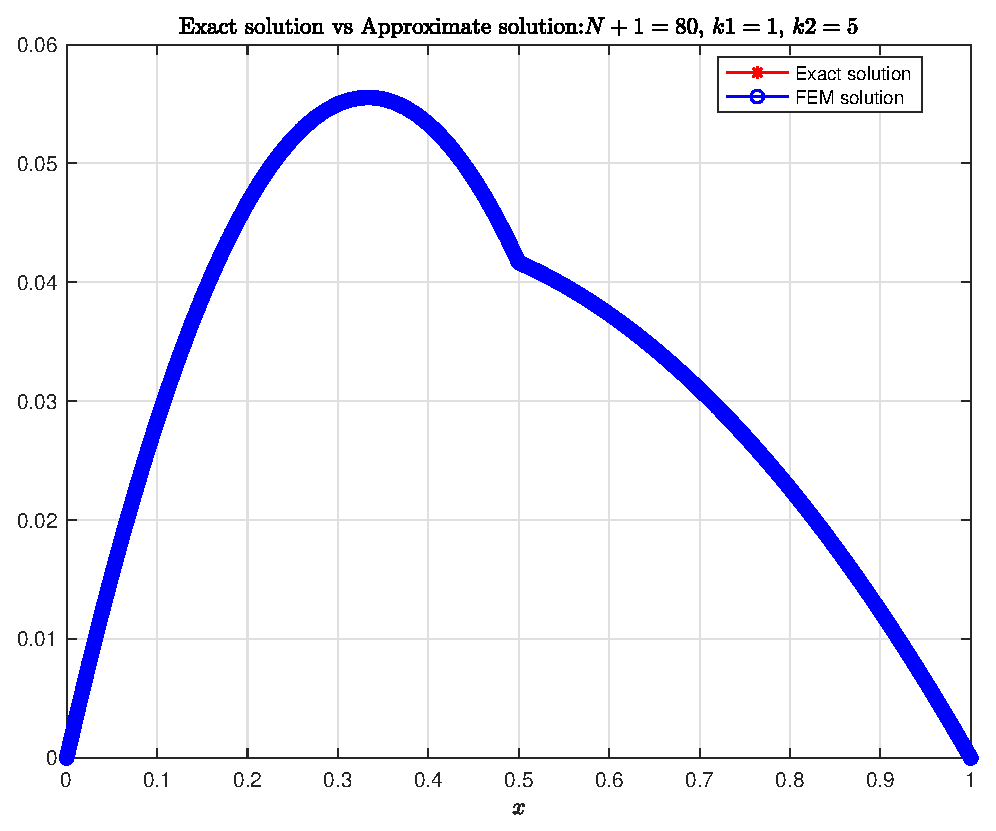
\includegraphics[width=0.29\textwidth]{img/solplot_N80_k11_k25.eps}
	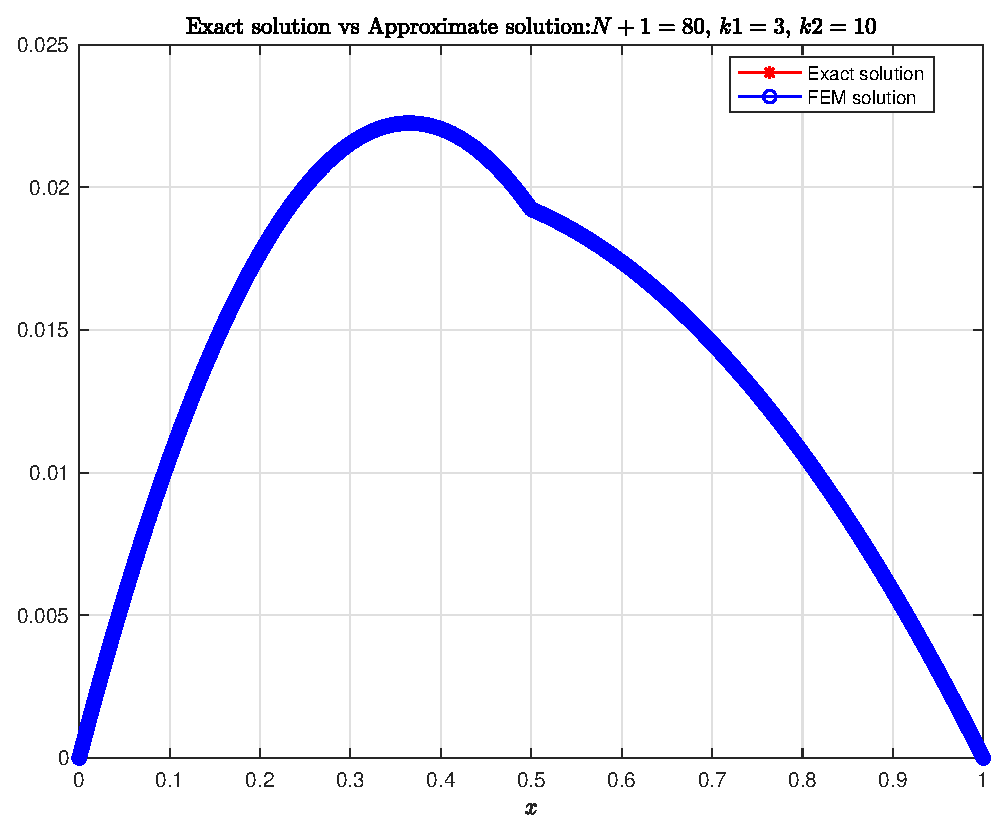
\includegraphics[width=0.29\textwidth]{img/solplot_N80_k13_k210.eps}
	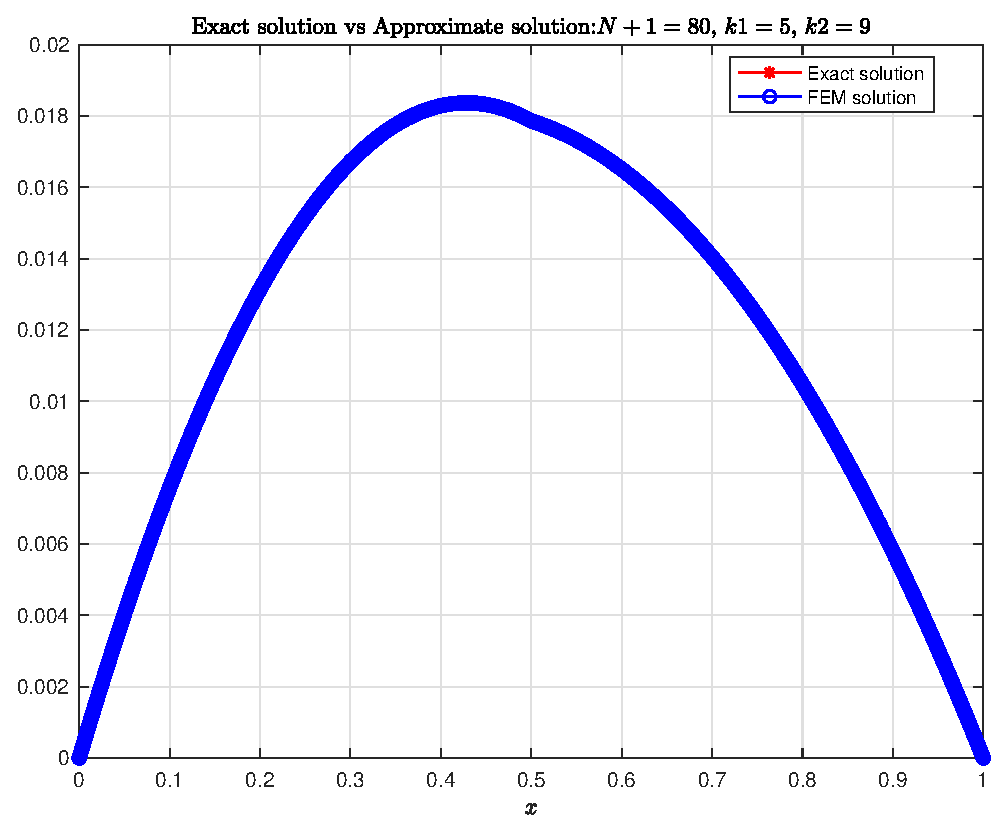
\includegraphics[width=0.29\textwidth]{img/solplot_N80_k15_k29.eps}
	\caption{Graph of FEM and Exact solution When $x_k =0.5$ is a node}
	\label{fig:N1}
\end{figure}
This is the result for the variant if the interface is not aligned with the mesh
\begin{table}[!h]
	\caption{Errors and convergence orders for $k_1=1$, $k_2=5$ (Variant)}
	\vspace{0.1in}
	\centering
	\begin{tabular}{|c|c|c|c|c|}
		\hline
		$N+1$ & $||e_h||_{L^2}$ & Order & $||e_h||_{L^\infty}$ & Order \\
		\hline
		11  & 2.7733E-03 & --   & 6.2895E-03 & --   \\
		21  & 1.4381E-03 & 1.02 & 3.3510E-03 & 0.97 \\
		41  & 7.3268E-04 & 1.01 & 1.7326E-03 & 0.99 \\
		81  & 3.6985E-04 & 1.00 & 8.8137E-04 & 0.99 \\
		161 & 1.8582E-04 & 1.00 & 4.4456E-04 & 1.00 \\
		\hline
	\end{tabular}
	\label{tab:k1_1_k2_5_nonuniform}
\end{table}
\begin{table}[!h]
	\caption{Errors and convergence orders for $k_1=3$, $k_2=10$ (Variant)}
	\vspace{0.1in}
	\centering
	\begin{tabular}{|c|c|c|c|c|}
		\hline
		$N+1$ & $||e_h||_{L^2}$ & Order & $||e_h||_{L^\infty}$ & Order \\
		\hline
		11  & 7.4602E-04 & --   & 1.6745E-03 & --   \\
		21  & 3.8222E-04 & 1.03 & 8.7720E-04 & 1.00 \\
		41  & 1.9373E-04 & 1.02 & 4.4959E-04 & 1.00 \\
		81  & 9.7570E-05 & 1.01 & 2.2768E-04 & 1.00 \\
		161 & 4.8969E-05 & 1.00 & 1.1458E-04 & 1.00 \\
		\hline
	\end{tabular}
	\label{tab:k1_3_k2_10_nonuniform}
\end{table}
\begin{table}[!h]
	\caption{Errors and convergence orders for $k_1=5$, $k_2=9$ (Varaint)}
	\vspace{0.1in}
	\centering
	\begin{tabular}{|c|c|c|c|c|}
		\hline
		$N+1$ & $||e_h||_{L^2}$ & Order & $||e_h||_{L^\infty}$ & Order \\
		\hline
		11  & 2.6975E-04 & --   & 5.8623E-04 & --   \\
		21  & 1.2973E-04 & 1.13 & 2.8535E-04 & 1.11 \\
		41  & 6.4212E-05 & 1.05 & 1.4029E-04 & 1.06 \\
		81  & 3.2064E-05 & 1.02 & 6.9489E-05 & 1.03 \\
		161 & 1.6040E-05 & 1.01 & 3.4572E-05 & 1.02 \\
		\hline
	\end{tabular}
	\label{tab:k1_5_k2_9_nonuniform}
\end{table}
\clearpage
\begin{figure}[htbp]
	\centering
	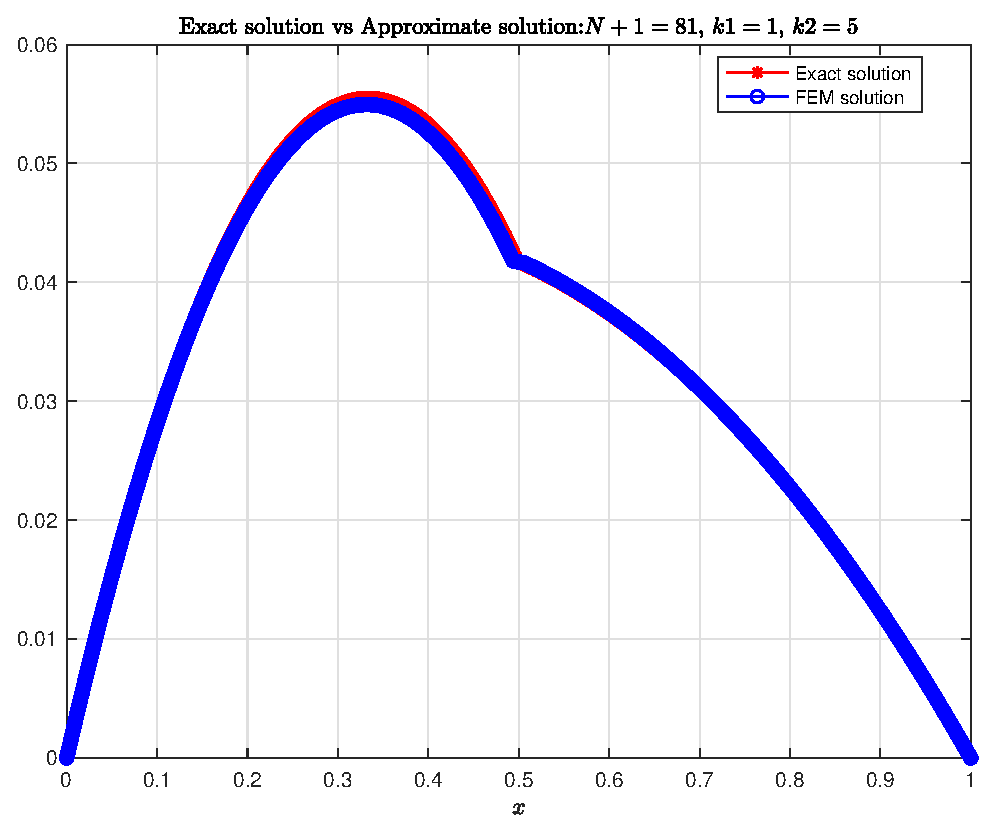
\includegraphics[width=0.29\textwidth]{img/bsolplot_N81_k11_k25.eps}
	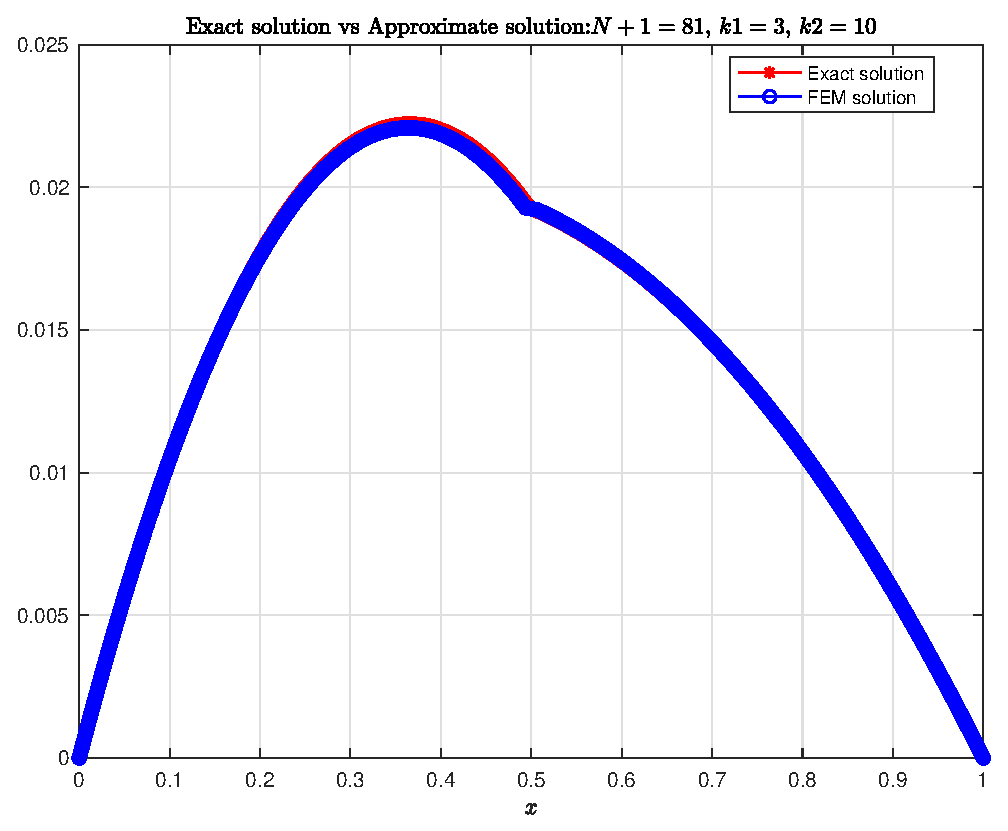
\includegraphics[width=0.29\textwidth]{img/bsolplot_N81_k13_k210.eps}
	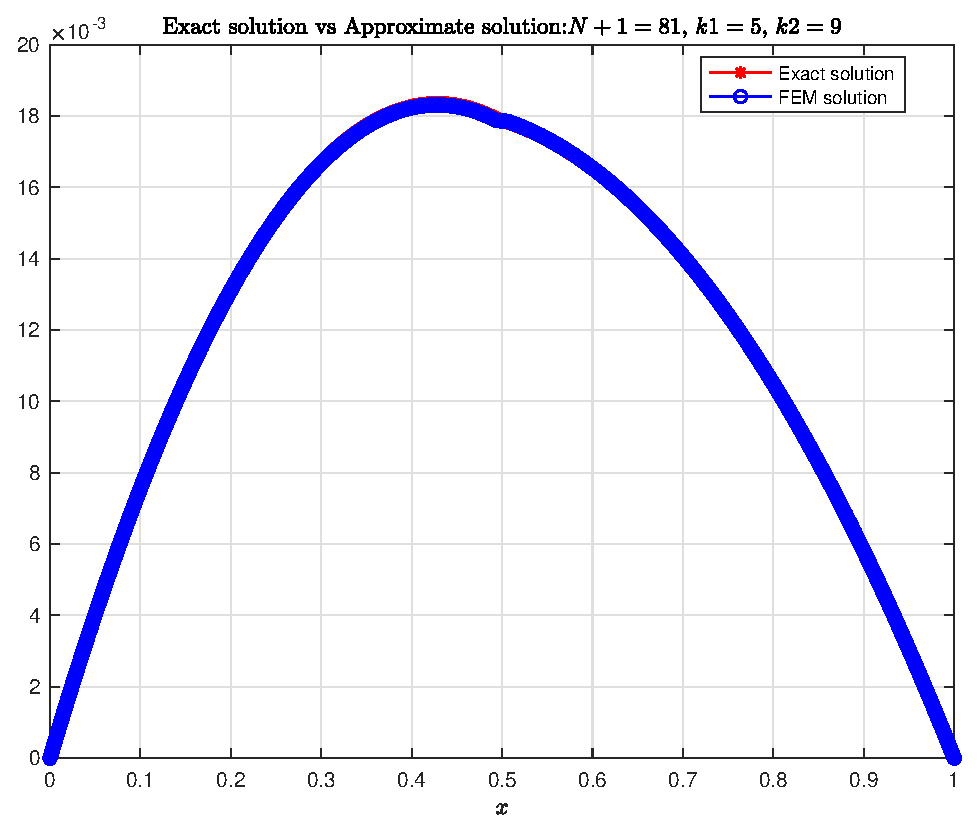
\includegraphics[width=0.29\textwidth]{img/bsolplot_N81_k15_k29.eps}
	\caption{Graph of FEM and Exact solution When $x_k =0.5$ does not align with the mesh}
	\label{fig:sN1}
\end{figure}
The numerical experiments clearly shows the effect of interface alignment on the accuracy and convergence of the finite element method for the given interface problem.
When the interface location $x = 0.5$ is aligned with mesh nodes, the finite element solution convergence rates aligns with the theory. In particular,
the $L^2$ and $L^\infty$ error shows second-order convergence, This is expected, since the mesh exactly resolves the discontinuity in the derivative of the solution at a nodal point.
In contrast, when the interface point $x = 0.5$ does not coincide with a mesh node, the convergence rates is approximately first order in both
$L^2$ and $L^\infty$ norms. In this case, the interface lies between an element. The element containing the interface becomes the dominant source of error, which limits the overall accuracy of the method.
These results highlight the importance of mesh alignment in interface problems.
\clearpage
\item[(a)] Mesh Type used for the implementation
\begin{figure}[htbp]
	\centering
	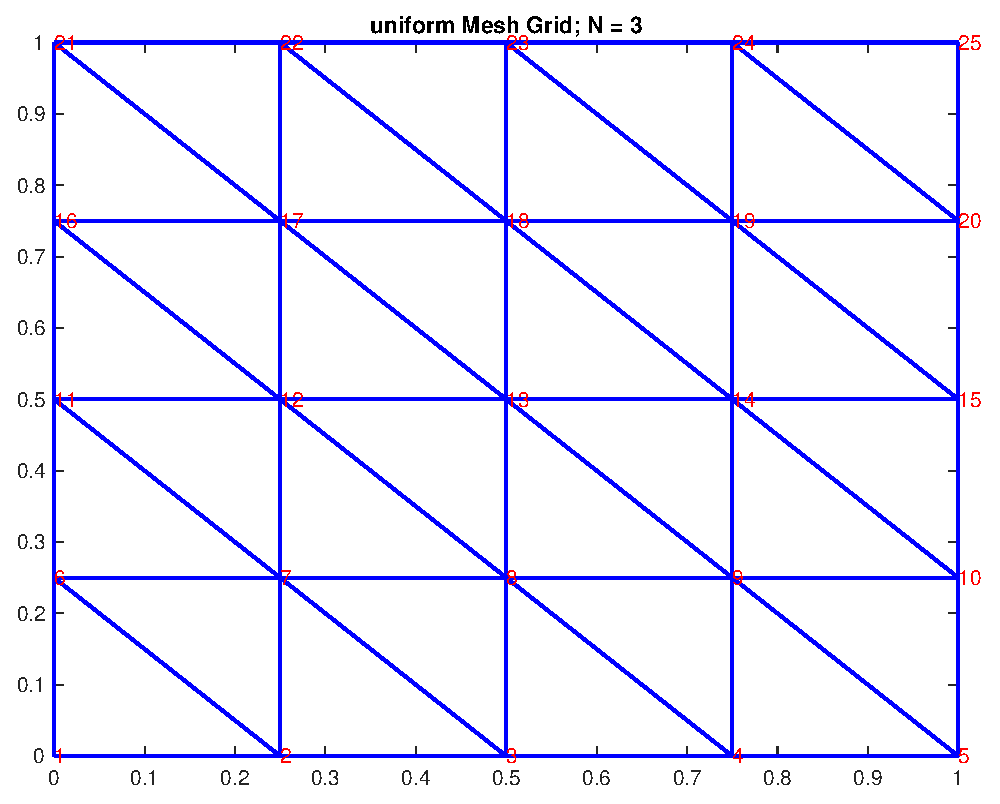
\includegraphics[width=0.4\textwidth]{img/mesh_uniform.eps}
	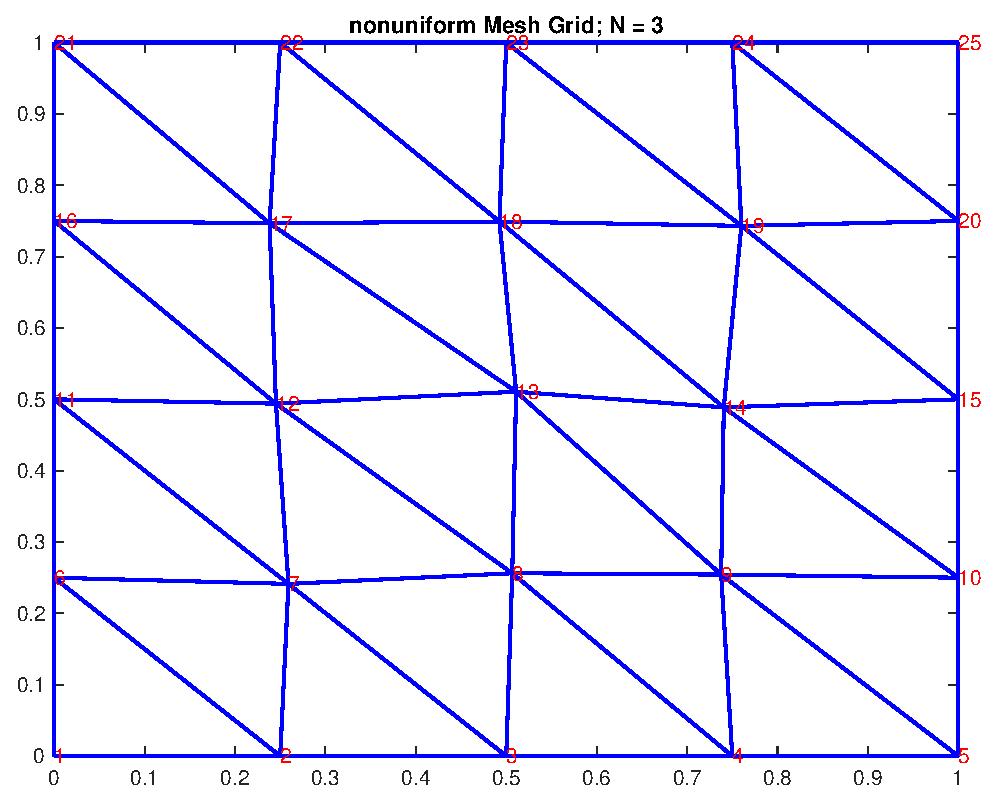
\includegraphics[width=0.4\textwidth]{img/mesh_nonuniform.eps}
%	
\includegraphics[width=0.55\textwidth]{img/solplot_N100_eps0.01.eps}
	\label{fig:N3}
\end{figure}
\item[(b)] The code is Implemented with a uniform mesh $h_j = h = \frac{1}{N+1}$, $p(x,y) = 3, \; q(x,y)=2$.  The exact solution is given by 
$$u(x,y) = 1, x, y$$ with it's  forcing  respectively given as 
$$f(x,y) =  2,2x,2y.$$
%\begin{figure}[htbp]
%	\centering
%	
\includegraphics[width=0.55\textwidth]{img/solplot_N10_eps0.5.eps}
%	
\includegraphics[width=0.55\textwidth]{img/solplot_N10_eps0.01.eps}
%	
\includegraphics[width=0.55\textwidth]{img/solplot_N100_eps0.01.eps}
%	\label{fig:N3}
%\end{figure}
\begin{table}[!h]
	\caption{$L^2$ Errors for uniform mesh}
	\vspace{0.1in}
	\centering
	\begin{tabular}{|c|c|c|c|}
		\hline
		& $u(x,y)=1$ & $u(x,y)=x$ & $u(x,y)=y$\\
		\hline
		$N+1$ & $||e_h(\cdot)||_{L^2(\Omega)}$ & $||e_h(\cdot)||_{L^2(\Omega)}$ & $||e_h(\cdot)||_{L^2(\Omega)}$\\
		\hline
		20    & 3.8773E-15   & 2.3988E-15    & 2.2512E-15\\
		40   & 2.4440E-14  & 1.2744E-14 & 1.2961E-14\\
		\hline
	\end{tabular}
	\label{tab1}
\end{table}
\begin{table}[!h]
	\caption{$L^2$ Errors for nonuniform mesh}
	\vspace{0.1in}
	\centering
	\begin{tabular}{|c|c|c|c|}
		\hline
		& $u(x,y)=1$ & $u(x,y)=x$ & $u(x,y)=y$\\
		\hline
		$N+1$ & $||e_h(\cdot)||_{L^2(\Omega)}$ & $||e_h(\cdot)||_{L^2(\Omega)}$ & $||e_h(\cdot)||_{L^2(\Omega)}$\\
		\hline
		20    & 6.716E-16   & 2.991E-16     & 6.021E-16\\
		40   & 3.259E-15  & 1.927E-15 & 8.246E-16\\
		\hline
	\end{tabular}
	\label{tab2}
\end{table}
\item[(c)] For exact solution, $u(x,y) = y^3 + \sin(5(x+y)) + 2e^x$. The partial derivatives are given below
\begin{align*}
	&u_x(x,y) = 5\cos(5(x+y)) + 2e^x,\\
	&u_{xx}(x,y) = -25\sin(5(x+y)) + 2e^x,\\
	&u_y(x,y)= 3y^2 + 5\cos(5(x+y)), \\
	&u_{yy}(x,y) = 6y -25\sin(5(x+y)).
\end{align*}
\begin{table}[!h]
	\caption{Errors, convergence orders, and computational time for uniform mesh}
	\vspace{0.1in}
	\centering
	\begin{tabular}{|c|c|c|c|c|c|c|}
		\hline
		$N+1$ & $||e_h||_{L^2}$ & Order & $||e_h||_{H^1}$ & Order & Assembly Time (s) & Solve Time (s) \\
		\hline
		10   & 2.9578E-02 & --    & 7.4805E-01 & --    & 8.8325E-03 & 1.4913E-04 \\
		20   & 7.5020E-03 & 1.98  & 3.7355E-01 & 1.00  & 9.4547E-03 & 2.6960E-03 \\
		40   & 1.8824E-03 & 1.99  & 1.8670E-01 & 1.00  & 3.1137E-02 & 2.3372E-02 \\
		80   & 4.7104E-04 & 2.00  & 9.3340E-02 & 1.00  & 1.2474E-01 & 4.7815E-01 \\
		160  & 1.1779E-04 & 2.00  & 4.6669E-02 & 1.00  & 5.3350E-01 & 3.0517E+01 \\
		\hline
	\end{tabular}
	\label{tab_fem_results_time}
\end{table}
\begin{table}[!h]
	\caption{Errors, convergence orders, and computational time for non-uniform mesh}
	\vspace{0.1in}
	\centering
	\begin{tabular}{|c|c|c|c|c|c|c|}
		\hline
		$N+1$ & $||e_h||_{L^2}$ & Order & $||e_h||_{H^1}$ & Order & Assembly Time (s) & Solve Time (s) \\
		\hline
		10   & 2.956E-02 & --    & 7.481E-01 & --    & 8.130E-03 & 1.405E-04 \\
		20   & 7.581E-03 & 1.96  & 3.751E-01 & 1.00  & 8.597E-03 & 2.274E-03 \\
		40   & 1.902E-03 & 2.00  & 1.875E-01 & 1.00  & 2.758E-02 & 1.849E-02 \\
		80   & 4.765E-04 & 2.00  & 9.380E-02 & 1.00  & 1.110E-01 & 5.115E-01 \\
		160  & 1.191E-04 & 2.00  & 4.689E-02 & 1.00  & 4.884E-01 & 3.930E+01 \\
		\hline
	\end{tabular}
	\label{tab_nonuniform_mesh}
\end{table}
\clearpage
\section{Conclusion}
The numerical results demonstrate that the finite element method achieves the expected optimal convergence rates for linear elements ($K \in P^1$). 
In particular, the $L^2$ error converges at approximately second order, $\mathcal{O}(h^2)$, while the $H^1$ error converges at first order, $\mathcal{O}(h)$. 
These rates are consistent with the theory for piecewise linear finite element approximations. 
A comparison between uniform and non-uniform meshes shows that both have the same convergence behavior. The non-uniform mesh does not affect the accuracy of the solution, 
and the convergence orders remain optimal in both norms.
The errors decrease smoothly as the mesh is refined. The behavior of the solution aligns well with theoretical expectations. 
For computation, the matrix assembly time increases moderately with the number of elements,
which is consistent with the expected linear scaling of element-wise assembly procedures. In contrast, the time required to solve the linear system grows rapidly as the problem size increases. This is due to the use of a directsolver, which becomes increasingly expensive for larger systems even when the matrix is sparse. As a result, the dominant computational cost shifts from assembly to the solution phase as the mesh is refined.
The primary limitation observed is computational efficiency at larger problem sizes, which could be improved by employing iterative solvers that better exploit the sparsity of the system matrix.
\end{enumerate}
\lstinputlisting[language=matlab, numbers=left, stepnumber=1, firstline=1,caption={main.m },label=code:main1,frame=single]{main.m}
\lstinputlisting[language=matlab, numbers=left, stepnumber=1, firstline=1,caption={Mesh generator.m },label=code:Meshgen,frame=single]{Meshgen.m}
\lstinputlisting[language=matlab, numbers=left, stepnumber=1, firstline=1,caption={twoPointBVP.m },label=code:main2,frame=single]{twoPointBVP2D.m}
\lstinputlisting[language=matlab, numbers=left, stepnumber=1, firstline=1,caption={formMatrix.m },label=code:main3,frame=single]{formMatrixEle.m}
\lstinputlisting[language=matlab, numbers=left, stepnumber=1, firstline=1,caption={$U_h (x,y)$ function },label=code:main4,frame=single]{UhElement.m}
\lstinputlisting[language=matlab, numbers=left, stepnumber=1, firstline=1,caption={$e_h(x,y)$ function },label=code:main5,frame=single]{getErrors.m}
\lstinputlisting[language=matlab, numbers=left, stepnumber=1, firstline=1,caption={main.m },label=code:main1D,frame=single]{1D problem/main.m}
\lstinputlisting[language=matlab, numbers=left, stepnumber=1, firstline=1,caption={twoPointBVP.m },label=code:twoP1D,frame=single]{1D problem/twoPointBVP.m}
\lstinputlisting[language=matlab, numbers=left, stepnumber=1, firstline=1,caption={formMatrix.m },label=code:main31,frame=single]{1D problem/formMatrix.m}
\lstinputlisting[language=matlab, numbers=left, stepnumber=1, firstline=1,caption={$U_h (x)$ function },label=code:main41,frame=single]{1D problem/UhFunc.m}
\lstinputlisting[language=matlab, numbers=left, stepnumber=1, firstline=1,caption={$U_{hx}(x)$ function },label=code:main51,frame=single]{1D problem/UhFuncx.m}
\section{Setup Description}

In this section, we describe the main components of the reduced basis (RB) method used for the parametrized problem.

\subsection{Spatial Discretization}

We consider the domain $[0,1]$ and discretize it using a uniform mesh with $N = 39$ interior nodes. The mesh is chosen such that the point $x = 0.5$ is included as a grid node, which is important due to the discontinuity in the reaction term.

\subsection{Parameter Domain}

The parameter vector is given by $\mu = (\mu_1, \mu_2) \in [0,1] \times [0,2]$.

\subsection{Training and Test Sets}

The training set $D_{\text{train}}$ is constructed as a uniform tensor grid over the parameter domain with $30 \times 30$ samples, resulting in a total of $900$ parameter points. This set is used in the greedy algorithm to construct the reduced basis.

The test set $D_{\text{test}}$ consists of $100$ randomly sampled parameters uniformly distributed over the parameter domain. It is used to evaluate the accuracy of the reduced model.

\subsection{Reduced Basis Construction}

The reduced basis is constructed using a greedy algorithm. Starting from an initial parameter value, the algorithm iteratively selects new parameters that maximize a chosen error indicator over the training set. The corresponding high-fidelity solutions are added to the basis.

Two variants of the basis are considered:
\begin{itemize}
	\item A direct basis formed by the collection of snapshots,
	\item An orthonormal basis obtained via QR decomposition.
\end{itemize}

\subsection{Error Estimation}

Two types of error indicators are used:
\begin{itemize}
	\item The $\ell^1$-norm of the reduced coefficients:
	\[
	\Delta(\mu) = \|c(\mu)\|_1,
	\]
	\item A residual-based estimator:
	\[
	\Delta(\mu) = \|f - A(\mu) u_m(\mu)\|.
	\]
\end{itemize}
The residual-based estimator provides a more reliable measure of the approximation error.

\subsection{Stopping Criterion}

The greedy algorithm is terminated when the maximum error indicator over the training set satisfies
\[
\max_{\mu \in D_{\text{train}}} \Delta(\mu) < 10^{-6},
\]
or when a maximum reduced basis size of $r_{\max} = 15$ is reached.

\subsection{Affine Decomposition and Precomputation}

The bilinear form admits an affine decomposition of the form
\[
A(\mu) = A_0 + \mu_1 A_1 + \mu_2 A_2.
\]
This structure enables an efficient offline-online decomposition. The matrices $A_0$, $A_1$, and $A_2$ are assembled during the offline stage, while reduced systems are solved efficiently during the online stage.
\end{document}               % End of document.
